\setcourse{数学分析II}
\setyear{2025\textasciitilde 2026}
\setterm{春季}
\settotal{4}
% \setexamtype{期末考试}

\begin{document}

\makeexamtitle

% \begin{xiaosihao}


\section{%
  选择题：本题共 5 小题, 每小题 3 分, 共 15 分。
  在每小题给出的四个选项中, 只有一项是符合题目要求的。
}

% \noindent\scoringbox


\begin{question}
设函数 $f(x)$ 在 $[0, 1]$ 上连续, $f(x) \geqslant 0$ 且 $\displaystyle \int_0^1 f(x) ~ \mathrm{d}x = 0.$ 则 \paren[A]

\begin{choices}
\item $f(x)$ 在 $[0, 1]$ 上恒等于零
\item $f(x)$ 在至多有限个点处非零
\item $f(x)$ 在 $(0, 1)$ 内必有零点, 但不恒为零
\item 以上都不对
\end{choices}
\end{question}

\begin{solution}
A. 若 $f(x_0) > 0$ 在某点 $x_0 \in [0, 1],$ 由连续性, 存在 $x_0$ 的邻域 $U$ 使 $f(x) > f(x_0)/2 > 0$ 在 $U$ 上, 从而 $\int_0^1 f \geqslant \int_U f > 0,$ 矛盾. 故 $f \equiv 0.$
\end{solution}

\begin{question}
以下正项级数中, 收敛的是 \paren[C]

\begin{choices}
\item $\displaystyle \sum_{n=2}^\infty \dfrac{1}{n \ln n}$
\item $\displaystyle \sum_{n=2}^\infty \dfrac{1}{n^{1 + 1/\ln n}}$
\item $\displaystyle \sum_{n=2}^\infty \dfrac{1}{n (\ln n)^2}$
\item $\displaystyle \sum_{n=1}^\infty \dfrac{1}{n^{1 + 1/n}}$
\end{choices}
\end{question}

\begin{solution}
A 发散: 由积分判别法, $\displaystyle\int_2^\infty \dfrac{\mathrm{d}x}{x \ln x} = \ln \ln x \big|_2^{+\infty} = +\infty.$

B 发散: $n^{1/\ln n} = e^{\ln n / \ln n} = e,$ 故 $\dfrac{1}{n^{1+1/\ln n}} = \dfrac{1}{en},$ 发散.

C 收敛: 由积分判别法, $\displaystyle\int_2^\infty \dfrac{\mathrm{d}x}{x(\ln x)^2} = \left[ -\dfrac{1}{\ln x} \right]_2^{+\infty} = \dfrac{1}{\ln 2} < +\infty.$

D 发散: $n^{1/n} = e^{(\ln n)/n} \to 1$ 故 $\dfrac{1}{n^{1+1/n}} \sim* \dfrac{1}{n},$ 发散.
\end{solution}

\begin{question}
设幂级数 $\displaystyle\sum_{n=0}^\infty a_n x^n$ 的收敛半径为 $R \in (0, +\infty).$ 以下说法正确的是 \paren[C]

\begin{choices}
\item 级数在 $(-R, R)$ 上一致收敛.
\item 若级数在收敛域的某端点处收敛, 则必然绝对收敛.
\item 对任意 $r \in (0, R),$ 级数在 $[-r, r]$ 上绝对收敛且一致收敛.
\item 若级数在 $x = -R$ 处收敛, 则其收敛域包含 $[-R, R].$
\end{choices}
\end{question}

\begin{solution}
A 错: 取 $\sum_{n=0}^\infty x^n$ ($R = 1$), 余项 $\displaystyle\frac{x^{N+1}}{1-x} \to +\infty$ 当 $x \to 1^-,$ 故级数在 $(-1, 1)$ 上不一致收敛.

B 错: 取 $\displaystyle\sum_{n=1}^\infty \frac{x^n}{n}$ ($R = 1$), 在 $x = -1$ 处 $\displaystyle\sum_{n=1}^\infty \frac{(-1)^n}{n}$ 条件收敛 (Leibniz 判别法), 非绝对收敛.

C 正确: 对 $|x| \leqslant r < R,$ 有 $|a_n x^n| \leqslant |a_n| r^n.$ 由收敛半径的定义, $\sum |a_n| r^n < +\infty.$ 由 Weierstrass $M$ 判别法, 级数在 $[-r, r]$ 上绝对收敛且一致收敛.

D 错: 取 $\displaystyle\sum_{n=1}^\infty \frac{x^n}{n}$ ($R = 1$), 在 $x = -1$ 处收敛, 但在 $x = 1$ 处 $\displaystyle\sum_{n=1}^\infty \frac{1}{n} = +\infty$ 发散, 故收敛域 $[-1, 1)$ 不包含 $[-1, 1].$
\end{solution}

\begin{question}
设二元函数 $f(x, y)$ 在点 $(x_0, y_0) \in \mathbb{R}^2$ 的某个去心邻域 $\mathring{O}((x_0, y_0), \delta)$ 内有定义, 且二次极限 $\lim\limits_{x \to x_0} \lim\limits_{y \to y_0} f(x,y) = 0.$ 那么以下说法\chemph{不正确}的是 \paren[A]

\begin{choices}
\item 若二次极限 $\lim\limits_{y \to y_0} \lim\limits_{x \to x_0} f(x,y) = 0,$ 则二重极限 $\lim\limits_{(x,y)\to(x_0,y_0)} f(x,y)$ 必然也存在.
\item 若二次极限 $\lim\limits_{y \to y_0} \lim\limits_{x \to x_0} f(x,y) = 1,$ 则二重极限 $\lim\limits_{(x,y)\to(x_0,y_0)} f(x,y)$ 必然不存在.
\item 若二重极限 $\lim\limits_{(x,y)\to(x_0,y_0)} f(x,y)$ 存在, 则必然等于 $0.$
\item 若二重极限 $\lim\limits_{(x,y)\to(x_0,y_0)} f(x,y)$ 存在, 则二次极限 $\lim\limits_{y \to y_0} \lim\limits_{x \to x_0} f(x,y)$ 可能存在也可能不存在.
\end{choices}
\end{question}

\begin{solution}
累次极限与重极限所有可能的取值情况如下:

\begin{table}[H]
\centering
\input{tables/multi-limits}
\end{table}

由此可知: A 不正确, 两个累次极限均存在且相等, 二重极限仍然可能不存在 (表中第 5 行).

B 正确: 若二重极限存在, 其值由任意趋近路径唯一确定, 故若两个累次极限均存在, 它们必然相等; 现在两者不等, 故二重极限不存在.

C 正确: 若二重极限 $L$ 存在, 则在任意路径下 $f \to L.$ 沿 $y = y_0$ 先固定再令 $y \to y_0$ 的路径推出 $L = 0.$

D 正确: 由表可知, 二重极限存在时, 两个累次极限不一定存在 (表中第 4 行).
\end{solution}

\begin{question}
设 $f_n(x)$ 在闭区间 $[a, b]$ 上连续, 函数项级数 $\sum_{n=1}^\infty f_n(x)$ 在 $[a, b]$ 上一致收敛于 $S(x).$ 以下说法\chemph{不正确}的是 \paren[A]

\begin{choices}
\item 若每个 $f_n(x)$ 在 $[a, b]$ 上可微, 则必有 $\displaystyle S'(x) = \sum_{n=1}^\infty f_n'(x).$
\item $S(x)$ 在 $[a, b]$ 上连续.
\item $\displaystyle\int_a^b S(x) ~ \mathrm{d}x = \sum_{n=1}^\infty \int_a^b f_n(x) ~ \mathrm{d}x.$
\item 对任意 $x_0 \in [a, b]$ 及趋于 $x_0$ 的数列 $\{x_m\} \subset* [a, b],$ 有 $\displaystyle\lim_{m \to \infty} S(x_m) = S(x_0).$
\end{choices}
\end{question}

\begin{solution}
A 不正确: 仅凭 $\sum f_n(x)$ 一致收敛不足以保证逐项求导合法, 还需要导函数级数 $\sum f_n(x)'$ 也一致收敛. 反例: 取 $f_n(x) = \sin(nx) / (n\sqrt{n}),$ $x \in [0, 1]$ 上. 因 $|f_n(x)| \leqslant n^{-3/2},$ Weierstrass 判别法保证 $\sum f_n$ 一致收敛. 但 $f_n'(x) = \cos(nx) / \sqrt{n},$ 而 $\sum f_n'(0) = \sum 1/\sqrt{n}$ 发散, 故逐项求导公式不成立.

B 正确: 一致收敛的连续函数级数的和函数是连续函数.

C 正确: 由一致收敛性可逐项积分.

D 正确: D 等价于 $S(x)$ 在 $x_0$ 处连续, 由 B 成立.
\end{solution}


\section{填空题：本题共 5 小题, 每小题 3 分, 共 15 分。}

\examsetup{
  question/index = 1
}

% \noindent\scoringbox

\begin{question}
$\int_{-\pi}^{\pi} \ln \left( \frac{\sqrt{x^2 + 2026} + x}{\sqrt{x^2 + 2026} - x} \right) ~ \mathrm{d}x =$\fillin [$0$].
\end{question}

\begin{solution}
被积函数是个奇函数, 所以在关于原点对称的区间 $[-\pi, \pi]$ 上积分值为 $0.$
\end{solution}


\begin{question}
使得反常积分 $\displaystyle \int_2^{+\infty} \dfrac{\mathrm{d}x}{x^s \ln^2 x}$ 收敛的实数 $s$ 的取值范围为 \fillin[$s \geqslant 1$].
\end{question}

\begin{solution}
当 $s > 1$ 时, 被积函数 $1/(x^s \ln^2 x) \leqslant 1/x^s,$ 故积分收敛.

当 $s = 1$ 时, $\displaystyle\int_2^{+\infty} \dfrac{\mathrm{d}x}{x \ln^2 x} = \left[ -\dfrac{1}{\ln x} \right]_2^{+\infty} = \dfrac{1}{\ln 2} < +\infty,$ 收敛.

当 $s < 1$ 时, 取 $\varepsilon = (1-s)/2 > 0.$ 对充分大的 $x,$ $\ln x \leqslant x^\varepsilon,$ 故 $\dfrac{1}{x^s \ln^2 x} \geqslant \dfrac{1}{x^{s+2\varepsilon}} = \dfrac{1}{x^{(1+s)/2}}.$ 由于 $(1+s)/2 < 1,$ $\int_2^\infty x^{-(1+s)/2}\,\mathrm{d}x$ 发散, 故原积分发散.

综上, 收敛的充要条件为 $s \geqslant 1.$
\end{solution}


\begin{question}
无穷乘积 $\prod_{n=2}^{\infty} \cos \frac{\pi}{2^n} =$ \fillin[$\frac{2}{\pi}$].
\end{question}

\begin{solution}
令 $x = \frac{\pi}{2},$ 并记 $p_n = \cos \dfrac{x}{2^n}.$ 则 $\lim\limits_{n \to \infty} p_n = \cos 0 = 1,$ 无穷乘积收敛的必要条件满足.

计算部分积 $P_n = \prod_{k=1}^n \cos \dfrac{x}{2^k}.$ 利用二倍角公式 $\sin\theta \cos\theta = \dfrac{1}{2}\sin 2\theta,$ 注意到
\begin{align*}
\sin\frac{x}{2^n} \cdot P_n
&= \cos\frac{x}{2} \cdot \cos\frac{x}{4} \cdots \left( \cos\frac{x}{2^n} \cdot \sin\frac{x}{2^n} \right)
= \cos\frac{x}{2} \cdot \cos\frac{x}{4} \cdots \cos\frac{x}{2^{n-1}} \cdot \frac{1}{2}\sin\frac{x}{2^{n-1}} \\
&\quad \vdots \\
&= \cos\frac{x}{2} \cdot \frac{1}{2^{n-1}}\sin\frac{x}{2} = \frac{1}{2^n}\sin x.
\end{align*}
故对所有正整数 $n$ 均有 $\sin\dfrac{x}{2^n} \cdot P_n = \dfrac{\sin x}{2^n}.$ 当 $n$ 充分大时 $\dfrac{x}{2^n} \to 0,$ $\sin\dfrac{x}{2^n} \neq 0,$ 从而
\[
P_n = \frac{\sin x}{2^n \sin\dfrac{x}{2^n}} = \frac{\sin x}{x} \cdot \frac{x/2^n}{\sin(x/2^n)} \xrightarrow[]{n\to\infty} \frac{\sin x}{x},
\]
上式最后的取极限成立是因为 $\dfrac{t}{\sin t} \to 1$ 当 $t \to 0.$ 故无穷乘积收敛且
\[
\prod_{n=1}^\infty \cos \dfrac{x}{2^n} = \dfrac{\sin x}{x}.
\]
将 $x = \frac{\pi}{2}$ 代回上式即有
\[
\prod_{n=2}^{\infty} \cos \frac{\pi}{2^n} = \prod_{n=1}^\infty \cos \dfrac{x}{2^n} = \dfrac{\sin x}{x} = \frac{1}{\pi/2} = \frac{2}{\pi}.
\]
\end{solution}


\begin{question}
$\displaystyle\lim_{n\to\infty} \frac{1}{n}\sum_{k=1}^n \frac{n^2}{n^2+k^2} =$ \fillin[$\dfrac{\pi}{4}$].
\end{question}

\begin{solution}
注意到 $\dfrac{n^2}{n^2+k^2} = \dfrac{1}{1+(k/n)^2},$ 故
\begin{equation*}
\frac{1}{n}\sum_{k=1}^n \frac{n^2}{n^2+k^2} = \frac{1}{n}\sum_{k=1}^n \frac{1}{1+(k/n)^2}
\end{equation*}
是函数 $f(x) = \dfrac{1}{1+x^2}$ 在 $[0, 1]$ 上以右端点为标记点的 Riemann 和. 由定积分的定义,
\begin{equation*}
\lim_{n\to\infty} \frac{1}{n}\sum_{k=1}^n \frac{n^2}{n^2+k^2} = \int_0^1 \frac{\mathrm{d}x}{1+x^2} = \arctan x\,\Big|_0^1 = \frac{\pi}{4}.
\end{equation*}
\end{solution}


\begin{question}
摆线 $x = t - \sin t,$ $y = 1 - \cos t$ ($0 \leqslant t \leqslant 2\pi$) 与 $x$ 轴围成的图形的面积为 \fillin[$3\pi$].
\end{question}

\begin{solution}
\begin{equation*}
S = \int_0^{2\pi} y ~ \mathrm{d}x = \int_0^{2\pi} (1 - \cos t)^2 ~ \mathrm{d}t = \int_0^{2\pi} \left(1 - 2\cos t + \cos^2 t\right) \mathrm{d}t = 2\pi - 0 + \pi = 3\pi.
\end{equation*}
\begin{center}
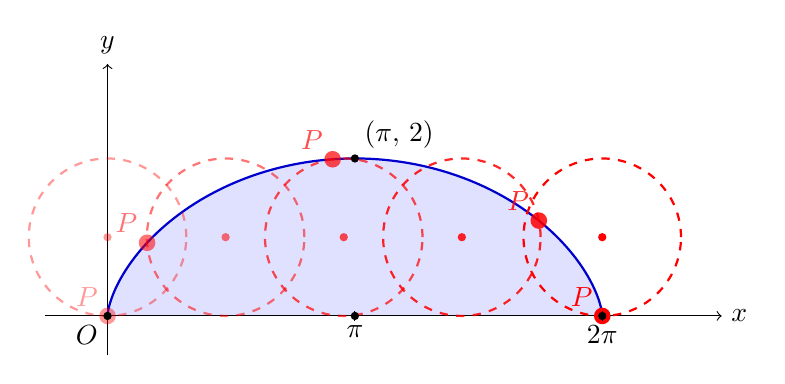
\begin{tikzpicture}[
declare function={
    cx(\t) = \t - sin(\t r);
    cy(\t) = 1 - cos(\t r);
}
]
% ---- 填充阴影区域 ----
\fill[blue!12]
    plot[domain=0:6.283185, samples=500, variable=\t]
        ({cx(\t)},{cy(\t)})
    -- cycle;

% ---- 画 x 轴 ----
\draw[->] (-0.8, 0) -- (7.8, 0) node[right] {$x$};
% ---- 画 y 轴 ----
\draw[->] (0, -0.5) -- (0, 3.2) node[above] {$y$};

% ---- 画摆线 ----
\draw[thick, blue!80!black]
    plot[domain=0:6.283185, samples=500, variable=\t]
        ({cx(\t)},{cy(\t)});

% ---- 画滚动的圆 ----
\foreach \xat in {0, 1.5, 3, 4.5, {2*pi}} {
    % 计算圆心和点P的位置
    \pgfmathsetmacro{\xcenter}{\xat}
    \pgfmathsetmacro{\ycenter}{1}
    \pgfmathsetmacro{\px}{cx(\xat)}
    \pgfmathsetmacro{\py}{cy(\xat)}

    % 画圆（透明度随t增加而降低）
    \pgfmathsetmacro{\opacity}{0.4 + \xat/10}
    \draw[red, thick, dashed, opacity=\opacity] (\xcenter, \ycenter) circle (1);

    % 标注圆心O'
    \fill[red, opacity=\opacity] (\xcenter, \ycenter) circle (1.5pt);

    % 标注点P
    \fill[red, opacity=\opacity] (\px, \py) circle (3pt) node[above left] {$P$};
}

% ---- 关键点标注 ----
\fill (0,0) circle (1.5pt) node[below left]  {$O$};
\fill ({pi},0) circle (1.5pt) node[below]      {$\pi$};
\fill ({2*pi},0) circle (1.5pt) node[below] {$2\pi$};
\fill ({pi},2) circle (1.5pt) node[above right] {$(\pi,\,2)$};

% ---- x 轴刻度 ----
\draw ({pi},0.06) -- ({pi},-0.06);
\draw ({2*pi},0.06) -- ({2*pi},-0.06);
\end{tikzpicture}
\end{center}

\end{solution}


\showquestionpoints

\section{计算题：本题共 2 小题, 共 20 分。本题应写出具体演算步骤。}

\examsetup{
  question/index = 1
}

\begin{question}[points = 10]
求幂级数 $\displaystyle\sum_{n=1}^\infty \dfrac{1}{(2n-1) \cdot 2^n} ~ x^{2n-1}$ 的收敛域及和函数.

% \noindent\scoringbox
\end{question}

\begin{solution}
记 $a_k = \begin{cases}
\frac{1}{(2n-1) \cdot 2^n}, & k = 2n-1, \\ 0, & k = 2n,
\end{cases}$ 则由 Cauchy-Hadamard 定理,
\[
\frac{1}{R} = \varlimsup_{k\to\infty} \sqrt[k]{a_k} = \varlimsup_{n\to\infty} \nroot[2n-1]{\frac{1}{(2n-1) \cdot 2^n}} = \frac{1}{\sqrt{2}}.
\]
故收敛半径 $R = \sqrt{2}.$ 在端点 $x = \pm\sqrt{2}$ 处, 通项化为 $\pm\dfrac{1}{(2n-1)\sqrt{2}} \to 0,$ 但 $\displaystyle\sum_{n=1}^\infty \dfrac{1}{(2n-1)\sqrt{2}}$ 与调和级数相比较发散, 故两端点处级数发散, 收敛域为 $(-\sqrt{2}, \sqrt{2}).$

令 $S(x) = \displaystyle\sum_{n=1}^\infty \dfrac{x^{2n-1}}{(2n-1) \cdot 2^n},$ 则 $S(0) = 0$ 且
\begin{equation*}
S'(x) = \sum_{n=1}^\infty \frac{x^{2(n-1)}}{2^n} = \frac{1}{2} \sum_{n=1}^\infty \left( \frac{x^2}{2} \right)^{n-1} = \frac{1}{2} \cdot \frac{1}{1 - x^2/2} = \frac{1}{2 - x^2}, \quad |x| < \sqrt{2}.
\end{equation*}
积分:
\begin{equation*}
S(x) = \int_0^x \frac{\mathrm{d}t}{2 - t^2} = \int_0^x \frac{\mathrm{d}t}{(\sqrt{2} + t)(\sqrt{2} - t)} = \frac{1}{2\sqrt{2}} \ln \frac{\sqrt{2} + x}{\sqrt{2} - x}, \quad x \in (-\sqrt{2}, \sqrt{2}).
\end{equation*}
\end{solution}


\begin{question}[points = 10]
计算 Cauchy 主值积分 $\displaystyle (\text{cpv}) \int_{-2}^2 \dfrac{1}{x^2 - 1} ~ \mathrm{d}x.$

% \noindent\scoringbox
\end{question}

\begin{solution}
被积函数 $f(x) = \dfrac{1}{x^2 - 1}$ 在积分区间 $[-2, 2]$ 上有两个奇点 $x = -1$ 和 $x = 1.$ 根据柯西主值的定义, 有
\begin{equation*}
(\text{cpv}) \int_{-2}^2 \frac{1}{x^2 - 1} ~ \mathrm{d}x = \lim_{\epsilon \to 0^+} \left( \int_{-2}^{-1-\epsilon} \frac{1}{x^2 - 1} ~ \mathrm{d}x + \int_{-1+\epsilon}^{1-\epsilon} \frac{1}{x^2 - 1} ~ \mathrm{d}x + \int_{1+\epsilon}^{2} \frac{1}{x^2 - 1} ~ \mathrm{d}x \right).
\end{equation*}
首先计算不定积分:
\begin{equation*}
\int \frac{1}{x^2 - 1} ~ \mathrm{d}x = \frac{1}{2} \int \left( \frac{1}{x-1} - \frac{1}{x+1} \right) ~ \mathrm{d}x = \frac{1}{2} \ln \left| \frac{x-1}{x+1} \right| + C.
\end{equation*}
将其代入各段积分中, 可得
\begin{align*}
\int_{-2}^{-1-\epsilon} \frac{1}{x^2 - 1} ~ \mathrm{d}x & = \frac{1}{2} \ln \left| \frac{x-1}{x+1} \right| \bigg|_{-2}^{-1-\epsilon} = \frac{1}{2} \left[ \ln \left( \frac{2+\epsilon}{\epsilon} \right) - \ln 3 \right].
\end{align*}
\begin{align*}
\int_{-1+\epsilon}^{1-\epsilon} \frac{1}{x^2 - 1} ~ \mathrm{d}x & = \frac{1}{2} \ln \left| \frac{x-1}{x+1} \right| \bigg|_{-1+\epsilon}^{1-\epsilon} = \frac{1}{2} \left[ \ln \left( \frac{\epsilon}{2-\epsilon} \right) - \ln \left( \frac{2-\epsilon}{\epsilon} \right) \right] \\
& = -\ln \left( \frac{2-\epsilon}{\epsilon} \right).
\end{align*}
\begin{align*}
\int_{1+\epsilon}^{2} \frac{1}{x^2 - 1} ~ \mathrm{d}x & = \frac{1}{2} \ln \left| \frac{x-1}{x+1} \right| \bigg|_{1+\epsilon}^{2} = \frac{1}{2} \left[ \ln \left( \frac{1}{3} \right) - \ln \left( \frac{\epsilon}{2+\epsilon} \right) \right] \\
& = \frac{1}{2} \left[ \ln \left( \frac{2+\epsilon}{\epsilon} \right) - \ln 3 \right].
\end{align*}
将上述三段结果相加, 得到
\begin{align*}
& \left( \int_{-2}^{-1-\epsilon} + \int_{-1+\epsilon}^{1-\epsilon} + \int_{1+\epsilon}^{2} \right) \frac{1}{x^2 - 1} ~ \mathrm{d}x \\
= & \frac{1}{2} \left[ \ln \left( \frac{2+\epsilon}{\epsilon} \right) - \ln 3 \right] - \ln \left( \frac{2-\epsilon}{\epsilon} \right) + \frac{1}{2} \left[ \ln \left( \frac{2+\epsilon}{\epsilon} \right) - \ln 3 \right] \\
= & \ln \left( \frac{2+\epsilon}{\epsilon} \right) - \ln \left( \frac{2-\epsilon}{\epsilon} \right) - \ln 3 \\
= & \ln(2+\epsilon) - \ln \epsilon - \ln(2-\epsilon) + \ln \epsilon - \ln 3 \\
= & \ln(2+\epsilon) - \ln(2-\epsilon) - \ln 3.
\end{align*}
令 $\epsilon \to 0^+,$ 则有
\begin{equation*}
(\text{cpv}) \int_{-2}^2 \frac{1}{x^2 - 1} ~ \mathrm{d}x = \lim_{\epsilon \to 0^+} [\ln(2+\epsilon) - \ln(2-\epsilon) - \ln 3] = \ln 2 - \ln 2 - \ln 3 = -\ln 3.
\end{equation*}
\end{solution}


\section{解答题：本题共 5 小题, 共 50 分。解答应写出文字说明或者证明过程。\chemph{注意，若一道题分为多个小问，则该题前面小问的结论可以用于后面的小问，但反过来不行}。}

\examsetup{
  question/index = 1
}

\begin{question}[points = 8]
设 $f(x)$ 为定义在 $(a, +\infty)$ 上的函数, 请叙述反常积分 $\int_a^{+\infty} f(x) ~ \mathrm{d}x$ 条件收敛的定义, 并给一个条件收敛的反常积分的例子.

% \noindent\scoringbox
\end{question}

\begin{solution}
反常积分 $\int_a^{+\infty} f(x) ~ \mathrm{d}x$ 条件收敛指的是 $\int_a^{+\infty} f(x) ~ \mathrm{d}x$ 收敛, 且  $\int_a^{+\infty} |f(x)| ~ \mathrm{d}x$ 发散. \score{4}

例子: $\int_0^{+\infty} \frac{\sin x}{x} ~ \mathrm{d} x.$ (不限于此例) \score{4}
\end{solution}


\begin{question}[points = 10]
设函数 $f: \mathbb{R}^2 \to \mathbb{R}$ 定义为
\[
f(x, y) = \begin{cases} \dfrac{x^2 y}{x^4 + y^2}, & (x, y) \neq (0, 0), \\ 0, & (x, y) = (0, 0). \end{cases}
\]
\begin{enumerate}
\item 证明: 对任意 $k \in \mathbb{R},$ 有 $\displaystyle\lim_{x \to 0} f(x, kx) = 0.$
\item 计算 $\displaystyle\lim_{x \to 0} f(x, x^2).$
\item 判断二重极限 $\displaystyle\lim_{(x,y) \to (0,0)} f(x,y)$ 是否存在, 并说明 $f$ 在原点处是否连续.
\end{enumerate}

% \noindent\scoringbox
\end{question}

\begin{solution}
\begin{enumerate}
\item 当 $k = 0$ 时, $f(x, 0) = 0$ 对一切 $x \neq 0$ 成立, 极限显然为 $0.$ 当 $k \neq 0$ 时,
\begin{equation*}
f(x, kx) = \frac{x^2 \cdot kx}{x^4 + k^2 x^2} = \frac{kx}{x^2 + k^2}.
\end{equation*}
由于 $\left|\dfrac{kx}{x^2 + k^2}\right| \leqslant \dfrac{|k| \cdot |x|}{k^2} = \dfrac{|x|}{|k|} \to 0$ 当 $x \to 0,$ 故 $\displaystyle\lim_{x\to 0} f(x, kx) = 0.$

\item 沿抛物线路径 $y = x^2$:
\begin{equation*}
f(x, x^2) = \frac{x^2 \cdot x^2}{x^4 + (x^2)^2} = \frac{x^4}{2x^4} = \frac{1}{2}, \quad x \neq 0.
\end{equation*}
故 $\displaystyle\lim_{x \to 0} f(x, x^2) = \dfrac{1}{2}.$

\item 由 (1), 沿任意过原点的直线趋近时极限为 $0;$ 由 (2), 沿抛物线 $y = x^2$ 趋近时极限为 $\dfrac{1}{2}.$ 两条路径给出不同的极限值, 故二重极限 $\displaystyle\lim_{(x,y)\to(0,0)} f(x,y)$ 不存在. 由于二重极限不存在, $f$ 在原点处不连续.
\end{enumerate}
\end{solution}


\begin{question}[points = 10]
设 $\{a_n\}$ 为正数列, 且正项级数 $\displaystyle\sum_{n=1}^\infty a_n$ 发散. 令 $S_n = \sum_{k=1}^n a_k.$ 证明: 级数 $\displaystyle\sum_{n=1}^\infty \dfrac{a_n}{S_n^2}$ 收敛.

% \noindent\scoringbox
\end{question}

\begin{solution}
由于 $S_n$ 单调递增, 对 $n \geqslant 2$ 有 $S_n \geqslant S_{n-1} > 0,$ 故
\begin{equation*}
\frac{a_n}{S_n^2} = \frac{S_n - S_{n-1}}{S_n^2} \leqslant \frac{S_n - S_{n-1}}{S_n \cdot S_{n-1}} = \frac{1}{S_{n-1}} - \frac{1}{S_n}.
\end{equation*}
对上式从 $n = 2$ 到 $N$ 求和, 得
\begin{equation*}
\sum_{n=2}^N \frac{a_n}{S_n^2} \leqslant \sum_{n=2}^N \left( \frac{1}{S_{n-1}} - \frac{1}{S_n} \right) = \frac{1}{S_1} - \frac{1}{S_N} \leqslant \frac{1}{S_1} = \frac{1}{a_1}.
\end{equation*}
由于各项非负且部分和有界, 正项级数 $\displaystyle\sum_{n=2}^\infty \dfrac{a_n}{S_n^2}$ 收敛, 从而 $\displaystyle\sum_{n=1}^\infty \dfrac{a_n}{S_n^2}$ 收敛.
\end{solution}


\begin{question}[points = 10]
设 $f: \mathbb{R}^n \rightarrow \mathbb{R}^m$ 是定义在 $\mathbb{R}^n$ 上取值在 $\mathbb{R}^m$ 中的连续向量值函数.
\begin{enumerate}
\item 设 $E \subset* \mathbb{R}^m$ 是 $\mathbb{R}^m$ 中开集. 请证明: $E$ 在 $f$ 下的原像
\[f^{-1}(E) = \{ x \in \mathbb{R}^n ~ : ~ f(x) \in E \}\]
必然是 $\mathbb{R}^n$ 中的开集.
\item 设 $F \subset* \mathbb{R}^n$ 是 $\mathbb{R}^n$ 中有界闭集. 请问 $F$ 在 $f$ 下的像
\[f(F) = \{ y \in \mathbb{R}^m ~ : ~ \exists ~ x \in F, ~ f(x) = y \}\]
是否必然是 $\mathbb{R}^m$ 中有界闭集? 若是, 请给出证明; 若否, 请给出反例.
\item 若 $F \subset* \mathbb{R}^n$ 仅是 $\mathbb{R}^n$ 中的闭集, 不一定有界. 请问这种情况下, $F$ 在 $f$ 下的像 $f(F)$ 是否仍必然是 $\mathbb{R}^m$ 中的闭集? 若是, 请给出证明; 若否, 请给出反例.
\end{enumerate}

% \noindent\scoringbox
\end{question}

\begin{solution}
\begin{enumerate}
\item 由开集的定义, 只要证明 $\forall ~ x \in f^{-1}(E),$ $x$ 是 $f^{-1}(E)$ 的内点即可:

由于 $E$ 是开集, 那么 $f(x) \in E$ 是 $E$ 的内点, 从而存在该点的邻域
\begin{equation*}
O(f(x), \varepsilon) = \{ y \in \mathbb{R}^m ~ : ~ d(y, f(x)) < \varepsilon \} \subset* E.
\end{equation*}
由于 $f$ 连续, 故对于取好的 $\varepsilon > 0,$ 存在 $\delta > 0,$ 使得对任意 $\widetilde{x} \in O(f(x), \delta),$ 总有 $d(f(\widetilde{x}), f(x)) < \varepsilon,$ 即 $f(\widetilde{x}) \in O(f(x), \varepsilon).$ 这表明
\begin{equation*}
f(O(x, \delta)) \subset* O(f(x), \varepsilon) \subset* E,
\end{equation*}
即有
\begin{equation*}
O(x, \delta) \subset* f^{-1}(E),
\end{equation*}
这就证明了 $x$ 是 $f^{-1}(E)$ 的内点.

\item $f(F)$ 必然是 $\mathbb{R}^m$ 中有界闭集. 原因如下:

欧氏空间中的集合是有界闭集, 与它是紧集是等价的. 我们只要验证 $f(F)$ 是紧集即可. 任取 $f(F)$ 的一个开覆盖
\begin{equation*}
f(F) \subset* \bigcup_{i \in I} U_i, ~ U_i \text{ 是 $\mathbb{R}^m$ 中开集}.
\end{equation*}
那么有 $\displaystyle F \subset* \bigcup_{i \in I} f^{-1}(U_i).$ 由第 (1) 问知, 由于 $f$ 连续, 故每一个 $f^{-1}(U_i)$ 都是 $\mathbb{R}^n$ 中开集, 即 $\displaystyle \bigcup_{i \in I} f^{-1}(U_i)$ 构成了 $F$ 的一个开覆盖. 由于 $F \subset* \mathbb{R}^n$ 是有界闭集, 即紧集, 可以从这个开覆盖中选出有限子覆盖
\begin{equation*}
F \subset* f^{-1}(U_{i_1}) \cup* f^{-1}(U_{i_2}) \cup* \cdots \cup* f^{-1}(U_{i_n}),
\end{equation*}
从而有
\begin{equation*}
f(F) \subset* U_{i_1} \cup* U_{i_2} \cup* \cdots \cup* U_{i_n}.
\end{equation*}
也就是说, 对 $f(F)$ 的任意开覆盖, 都可以从中选取出它的有限开覆盖, 故 $f(F)$ 是紧集, 即有界闭集.

\item 当 $F \subset* \mathbb{R}^n$ 是 $\mathbb{R}^n$ 中的无界闭集时, $f(F)$ 有可能不是 $\mathbb{R}^m$ 中的闭集. 例如 (不限于该例子):
\begin{equation*}
f: \mathbb{R} \rightarrow \mathbb{R}, ~ x \mapsto \dfrac{1}{x^2 + 1},
\end{equation*}
对于无界闭集 $F = [0, +\infty),$ 其像集 $f(F) = (0, 1]$ 不是闭集.
\end{enumerate}
\end{solution}


\begin{question}[points = 12]
考虑定义在 $s \in (1, +\infty)$ 上的 Riemann zeta 函数 $\displaystyle \zeta(s) := \sum_{n=1}^\infty \dfrac{1}{n^{s}}.$
\begin{enumerate}
\item 请证明: $\displaystyle \lim_{s \to +\infty} \zeta(s) = 1.$ (提示: 利用级数与积分的关系)
\item 已知在 $|x| < 1$ 范围内成立无穷乘积展开
\[
\dfrac{\sin \pi x}{\pi x} = \prod_{n=1}^\infty \left( 1 - \dfrac{x^2}{n^2} \right),
\]
请由此计算 $f(x) = \tan x$ 在 $x = 0$ 附近的幂级数展开, 并求其收敛半径. (提示: 对无穷乘积展开式取对数导数 $\displaystyle \dfrac{\mathrm{d}}{\mathrm{d} x} \left( \ln (\cdot) \right)$, 并利用恒等式 $\tan x = \cot x - 2\cot 2x$)
\item 求 $\zeta(2), \zeta(4)$ 的值.
\end{enumerate}

% \noindent\scoringbox
\end{question}

\begin{solution}
\begin{enumerate}
\item 对于 $s > 1$ 有
\begin{equation*}
1 \leqslant \zeta(s) = \sum_{n=1}^\infty \frac1{n^s} = 1 + \sum_{n=2}^\infty \frac1{n^s} \leqslant 1 + \sum_{n=2}^\infty \int_{n-1}^n \frac{1}{x^s} ~ \mathrm{d}x = 1 + \int_1^\infty \frac{1}{x^s} ~ \mathrm{d}x = 1 + \frac{1}{s-1}.
\end{equation*}
上式右端关于 $s \to +\infty$ 的极限等于 $1,$ 由夹逼准则知 $\displaystyle \lim_{s \to +\infty} \zeta(s) = 1.$ \score{5}

\item 对无穷乘积展开式两边取对数导数 $\displaystyle \dfrac{1}{\pi} \cdot \dfrac{\mathrm{d}}{\mathrm{d} x} \left( \ln (\cdot) \right)$ 有
\begin{equation*}
\dfrac{\cos \pi x}{\sin \pi x} - \dfrac{1}{\pi x}
= -\dfrac{1}{\pi} \sum_{n=1}^\infty \dfrac{2x}{n^2} \cdot \left( 1 - \dfrac{x^2}{n^2} \right)^{-1},
\end{equation*}
从而有
\begin{align*}
\pi x \cot \pi x
& = 1 - 2 \sum_{n=1}^\infty \dfrac{x^2}{n^2} \cdot \left( 1 - \dfrac{x^2}{n^2} \right)^{-1} = 1 - 2 \sum_{n=1}^\infty \dfrac{x^2}{n^2} \cdot \left( \sum_{k=0}^\infty \left( \dfrac{x^2}{n^2} \right)^k \right) \\
& = 1 - 2 \sum_{n=1}^\infty \sum_{k=1}^\infty \left( \dfrac{x^2}{n^2} \right)^k = 1 - 2 \sum_{k=1}^\infty \left( \sum_{n=1}^\infty \dfrac{1}{n^{2k}} \right) x^{2k} \\
& = 1 - 2 \sum_{k=1}^\infty \zeta(2k) x^{2k}.
\end{align*}
由此可求得
\begin{equation*}
\cot x = \dfrac{1}{x} - 2 \sum_{k=1}^\infty \dfrac{\zeta(2k)}{\pi^{2k}} x^{2k-1},
\end{equation*}
代入 $\tan x = \cot x - 2 \cot 2x$ 可得
\begin{equation*}
\tan x = 2 \sum_{k=1}^\infty \dfrac{(4^k - 1)\zeta(2k)}{\pi^{2k}} x^{2k-1}. \score{2}
\end{equation*}

进一步利用第 (1) 问证明的 $\displaystyle \lim_{n\to\infty} \zeta(n) = 1,$ 可得
\begin{equation*}
\dfrac{1}{R^2} = \lim_{k\to\infty} \dfrac{(4^{k+1} - 1)\zeta(2k+2)}{\pi^{2k+2}}
  \cdot \dfrac{\pi^{2k}}{(4^k - 1)\zeta(2k)}
= \dfrac{4}{\pi^2}, \score{2}
\end{equation*}
从而知 $\tan x$ 的收敛半径 $\displaystyle R = \dfrac{\pi}{2}.$ \score{1}

\item $\tan x$ 在 $x = 0$ 附近的 Taylor 级数为 $\displaystyle \tan x = \sum_{n=1}^\infty \dfrac{\tan^{(n)}(0)}{n!} x^n.$ 将其与第 (2) 问中求得的用 Riemann zeta 函数 $\zeta(s)$ 在 $s = 2, 4, \dots$ 处的特殊值表达的幂级数展开对比得
\begin{equation*}
\tan'(0) = \dfrac{2\cdot(4-1)}{\pi^2} \zeta(2) = \dfrac{6}{\pi^2} \zeta(2), \quad \dfrac{\tan^{(3)}(0)}{3!} = \dfrac{2\cdot(4^2-1)}{\pi^4} \zeta(4) = \dfrac{30}{\pi^4} \zeta(4).
\end{equation*}
容易算得
\begin{align*}
\tan'(0) & = \dfrac{1}{\cos^2x} \bigg|_{x=0} = 1, \\
\tan^{(3)}(0) & = \left.(4\sec^2 x \tan^2 x + 2\sec^4 x)\right|_{x=0} = 2,
\end{align*}
于是 \score{2}
\begin{align*}
\zeta(2) & = \dfrac{\pi^2}{6} \cdot \tan'(0) = \dfrac{\pi^2}{6}, \\
\zeta(4) & = \dfrac{\pi^4}{30} \cdot \dfrac{\tan^{(3)}(0)}{3!} = \dfrac{\pi^4}{90}.
\end{align*}
\end{enumerate}
\end{solution}

% \end{xiaosihao}

\end{document}
